% move all configuration stuff into includes file so we can focus on the content
\documentclass[aspectratio=169,hyperref={pdfpagelabels=false,colorlinks=true,linkcolor=white,urlcolor=lightblue},xcolor={table},t]{beamer}

%%%%%%%%%%%%%%%%%%%%%%%%%%%%%%%%%%%%%%%%%%%%%%%%%%%%%%%%%%%%%%%%%%%%%%%%%%%%%%%%%%
%%%%%%%%%%%%%%%%%%%%%%%%%%%%%%%%%%%%%%%%%%%%%%%%%%%%%%%%%%%%%%%%%%%%%%%%%%%%%%%%%%
% packages
\usepackage{pict2e}
\usepackage{epic}
\usepackage{amsmath,amsfonts,amssymb}
\usepackage{units}
\usepackage{fancybox}
\usepackage[absolute,overlay]{textpos} 
%\usepackage[table]{xcolor}
\usepackage{animate}
\usepackage{gensymb}
%\usepackage{graphicx}
%\usepackage{longtable}
\usepackage{multirow}
\usepackage{silence}
\usepackage{tikz}
\usepackage[backend=bibtex,style=ieee]{biblatex}
\AtEveryCitekey{\iffootnote{\tiny}{}}
\addbibresource{include/references}



% fontsize
\let\Tiny=\tiny

%%%%%%%%%%%%%%%%%%%%%%%%%%%%%%%%%%%%%%%%%%%%%%%%%%%%%%%%%%%%%%%%%%%%%%%%%%%%%%%%%%
%%%%%%%%%%%%%%%%%%%%%%%%%%%%%%%%%%%%%%%%%%%%%%%%%%%%%%%%%%%%%%%%%%%%%%%%%%%%%%%%%%
% warnings
\pdfsuppresswarningpagegroup=1
\WarningFilter{biblatex}{Patching footnotes failed}
\WarningFilter{latexfont}{Font shape}
\WarningFilter{latexfont}{Some font shapes}
\WarningFilter{gensymb}{Not defining}


%%%%%%%%%%%%%%%%%%%%%%%%%%%%%%%%%%%%%%%%%%%%%%%%%%%%%%%%%%%%%%%%%%%%%%%%%%%%%%%%%%
%%%%%%%%%%%%%%%%%%%%%%%%%%%%%%%%%%%%%%%%%%%%%%%%%%%%%%%%%%%%%%%%%%%%%%%%%%%%%%%%%%
% theme & layout
\usetheme{Frankfurt}
\useinnertheme{rectangles}


%%%%%%%%%%%%%%%%%%%%%%%%%%%%%%%%%%%%%%%%%%%%%%%%%%%%%%%%%%%%%%%%%%%%%%%%%%%%%%%%%%
\setbeamertemplate{frametitle}[default][colsep=-4bp,rounded=false,shadow=false]
\setbeamertemplate{frametitle}
{%
    \nointerlineskip%
    %\vskip-0.5ex
    \begin{beamercolorbox}[wd=\paperwidth,ht=3.5ex,dp=0.6ex]{frametitle}
        \hspace*{1.3ex}\insertframetitle%
        
        \hspace*{1.3ex}\small\insertframesubtitle%
    \end{beamercolorbox}%
    \begin{textblock*}{100mm}(13.75cm,1cm)
        
\includegraphics[height=.4cm,keepaspectratio]{graph/Logo_GTCMT_white}
    \end{textblock*}
}


%%%%%%%%%%%%%%%%%%%%%%%%%%%%%%%%%%%%%%%%%%%%%%%%%%%%%%%%%%%%%%%%%%%%%%%%%%%%%%%%%%
\setbeamertemplate{title page}[default][colsep=-4bp,rounded=false,shadow=false]
\setbeamertemplate{title page}
{
    \begin{textblock*}{100mm}(15cm,.51cm)
            \href{https://github.com/alexanderlerch/ACA-Slides/blob/2nd_edition/\jobname.pdf}{\includegraphics[height=.5cm,keepaspectratio]{graph/Logo_github}}\hspace*{2ex}
    \end{textblock*}
    \begin{textblock*}{100mm}(15cm,1.3cm)
            \href{\IEEELink}{
\includegraphics[height=.5cm,keepaspectratio]{graph/icon/book}}\hspace*{2ex}
    \end{textblock*}
    \vskip-10ex
    \begin{beamercolorbox}[wd=\paperwidth,ht=.7\paperheight,dp=0.6ex]{frametitle} %35ex
        %\begin{flushright}
            %\href{http://www.gtcmt.gatech.edu}{
\includegraphics[height=.8cm,keepaspectratio]{graph/Logo_GTCMT_black}}\hspace*{2ex}
        %\end{flushright}
        
        \hspace*{1.8ex}\LARGE\inserttitle%
        
        \vspace*{.5ex}
        
        \hspace*{1.3ex}\small\insertsubtitle%
        
        \vspace*{.5ex}
    \end{beamercolorbox}%
    \nointerlineskip%
    \begin{beamercolorbox}[wd=\paperwidth,ht=.4\paperheight,dp=0.6ex]{page number in head/foot}
        %\vspace*{-.5ex}
        \hspace*{1.7ex}\small\insertauthor%
        
        %\hspace*{1.7ex}\small }%
        
        \vspace*{12ex}
        \vfill
        \begin{flushright}
            \href{http://www.gtcmt.gatech.edu}{
\includegraphics[height=.5cm,keepaspectratio]{graph/Logo_GTCMT_black}}\hspace*{2ex}
        \end{flushright}
    \end{beamercolorbox}%
}


%%%%%%%%%%%%%%%%%%%%%%%%%%%%%%%%%%%%%%%%%%%%%%%%%%%%%%%%%%%%%%%%%%%%%%%%%%%%%%%%%%
%\makeatother
\setbeamertemplate{footline}
{
  \leavevmode%
  \hbox{%
  \begin{beamercolorbox}[wd=.5\paperwidth,ht=2.25ex,dp=1ex,left,leftskip=1ex]{page number in head/foot}%
    \insertsubtitle
  \end{beamercolorbox}%
  \begin{beamercolorbox}[wd=.5\paperwidth,ht=2.25ex,dp=1ex,right,rightskip=1ex]{page number in head/foot}%
    \hfill
    \insertframenumber{} / \inserttotalframenumber
  \end{beamercolorbox}}%
  \vskip0pt%
}
%\makeatletter


%%%%%%%%%%%%%%%%%%%%%%%%%%%%%%%%%%%%%%%%%%%%%%%%%%%%%%%%%%%%%%%%%%%%%%%%%%%%%%%%%%
\beamertemplatenavigationsymbolsempty
\setbeamertemplate{navigation symbols}{}
\setbeamertemplate{blocks}[default]%[rounded=false,shadow=false]
\setbeamertemplate{itemize item}[square]
\setbeamertemplate{itemize subitem}[circle]
\setbeamertemplate{itemize subsubitem}[triangle]
\setbeamertemplate{enumerate item}[square]
\setbeamertemplate{enumerate subitem}[circle]
\setbeamertemplate{enumerate subsubitem}[circle]


%%%%%%%%%%%%%%%%%%%%%%%%%%%%%%%%%%%%%%%%%%%%%%%%%%%%%%%%%%%%%%%%%%%%%%%%%%%%%%%%%%
% colors
\setbeamercolor{structure}{fg=darkgray}
\setbeamercovered{transparent} %invisible
\setbeamercolor{bibliography entry author}{fg=black}
\setbeamercolor*{bibliography entry title}{fg=black}
\setbeamercolor*{bibliography entry note}{fg=black}
\setbeamercolor{frametitle}{fg=black}
\setbeamercolor{title}{fg=white}
\setbeamercolor{subtitle}{fg=white}
\setbeamercolor{frametitle}{fg=white}
\setbeamercolor{framesubtitle}{fg=white}
\setbeamercolor{mini frame}{fg=white, bg=black}
\setbeamercolor{section in head/foot}{fg=white, bg=darkgray}
\setbeamercolor{page number in head/foot}{fg=black, bg=lightblue}
\setbeamercolor{item projected}{fg=white, bg=black}

%---------------------------------------------------------------------------------
%%%%%%%%%%%%%%%%%%%%%%%%%%%%%%%%%%%%%%%%%%%%%%%%%%%%%%%%%%%%%%%%%%%%%%%%%%%%%%%%%%
%%%%%%%%%%%%%%%%%%%%%%%%%%%%%%%%%%%%%%%%%%%%%%%%%%%%%%%%%%%%%%%%%%%%%%%%%%%%%%%%%%
% title information
\title[]{Introduction to \textbf{Audio Content Analysis}}   
\author[alexander lerch]{alexander lerch} 
%\institute{~}
%\date[Alexander Lerch]{}
%\titlegraphic{\vspace{-16mm}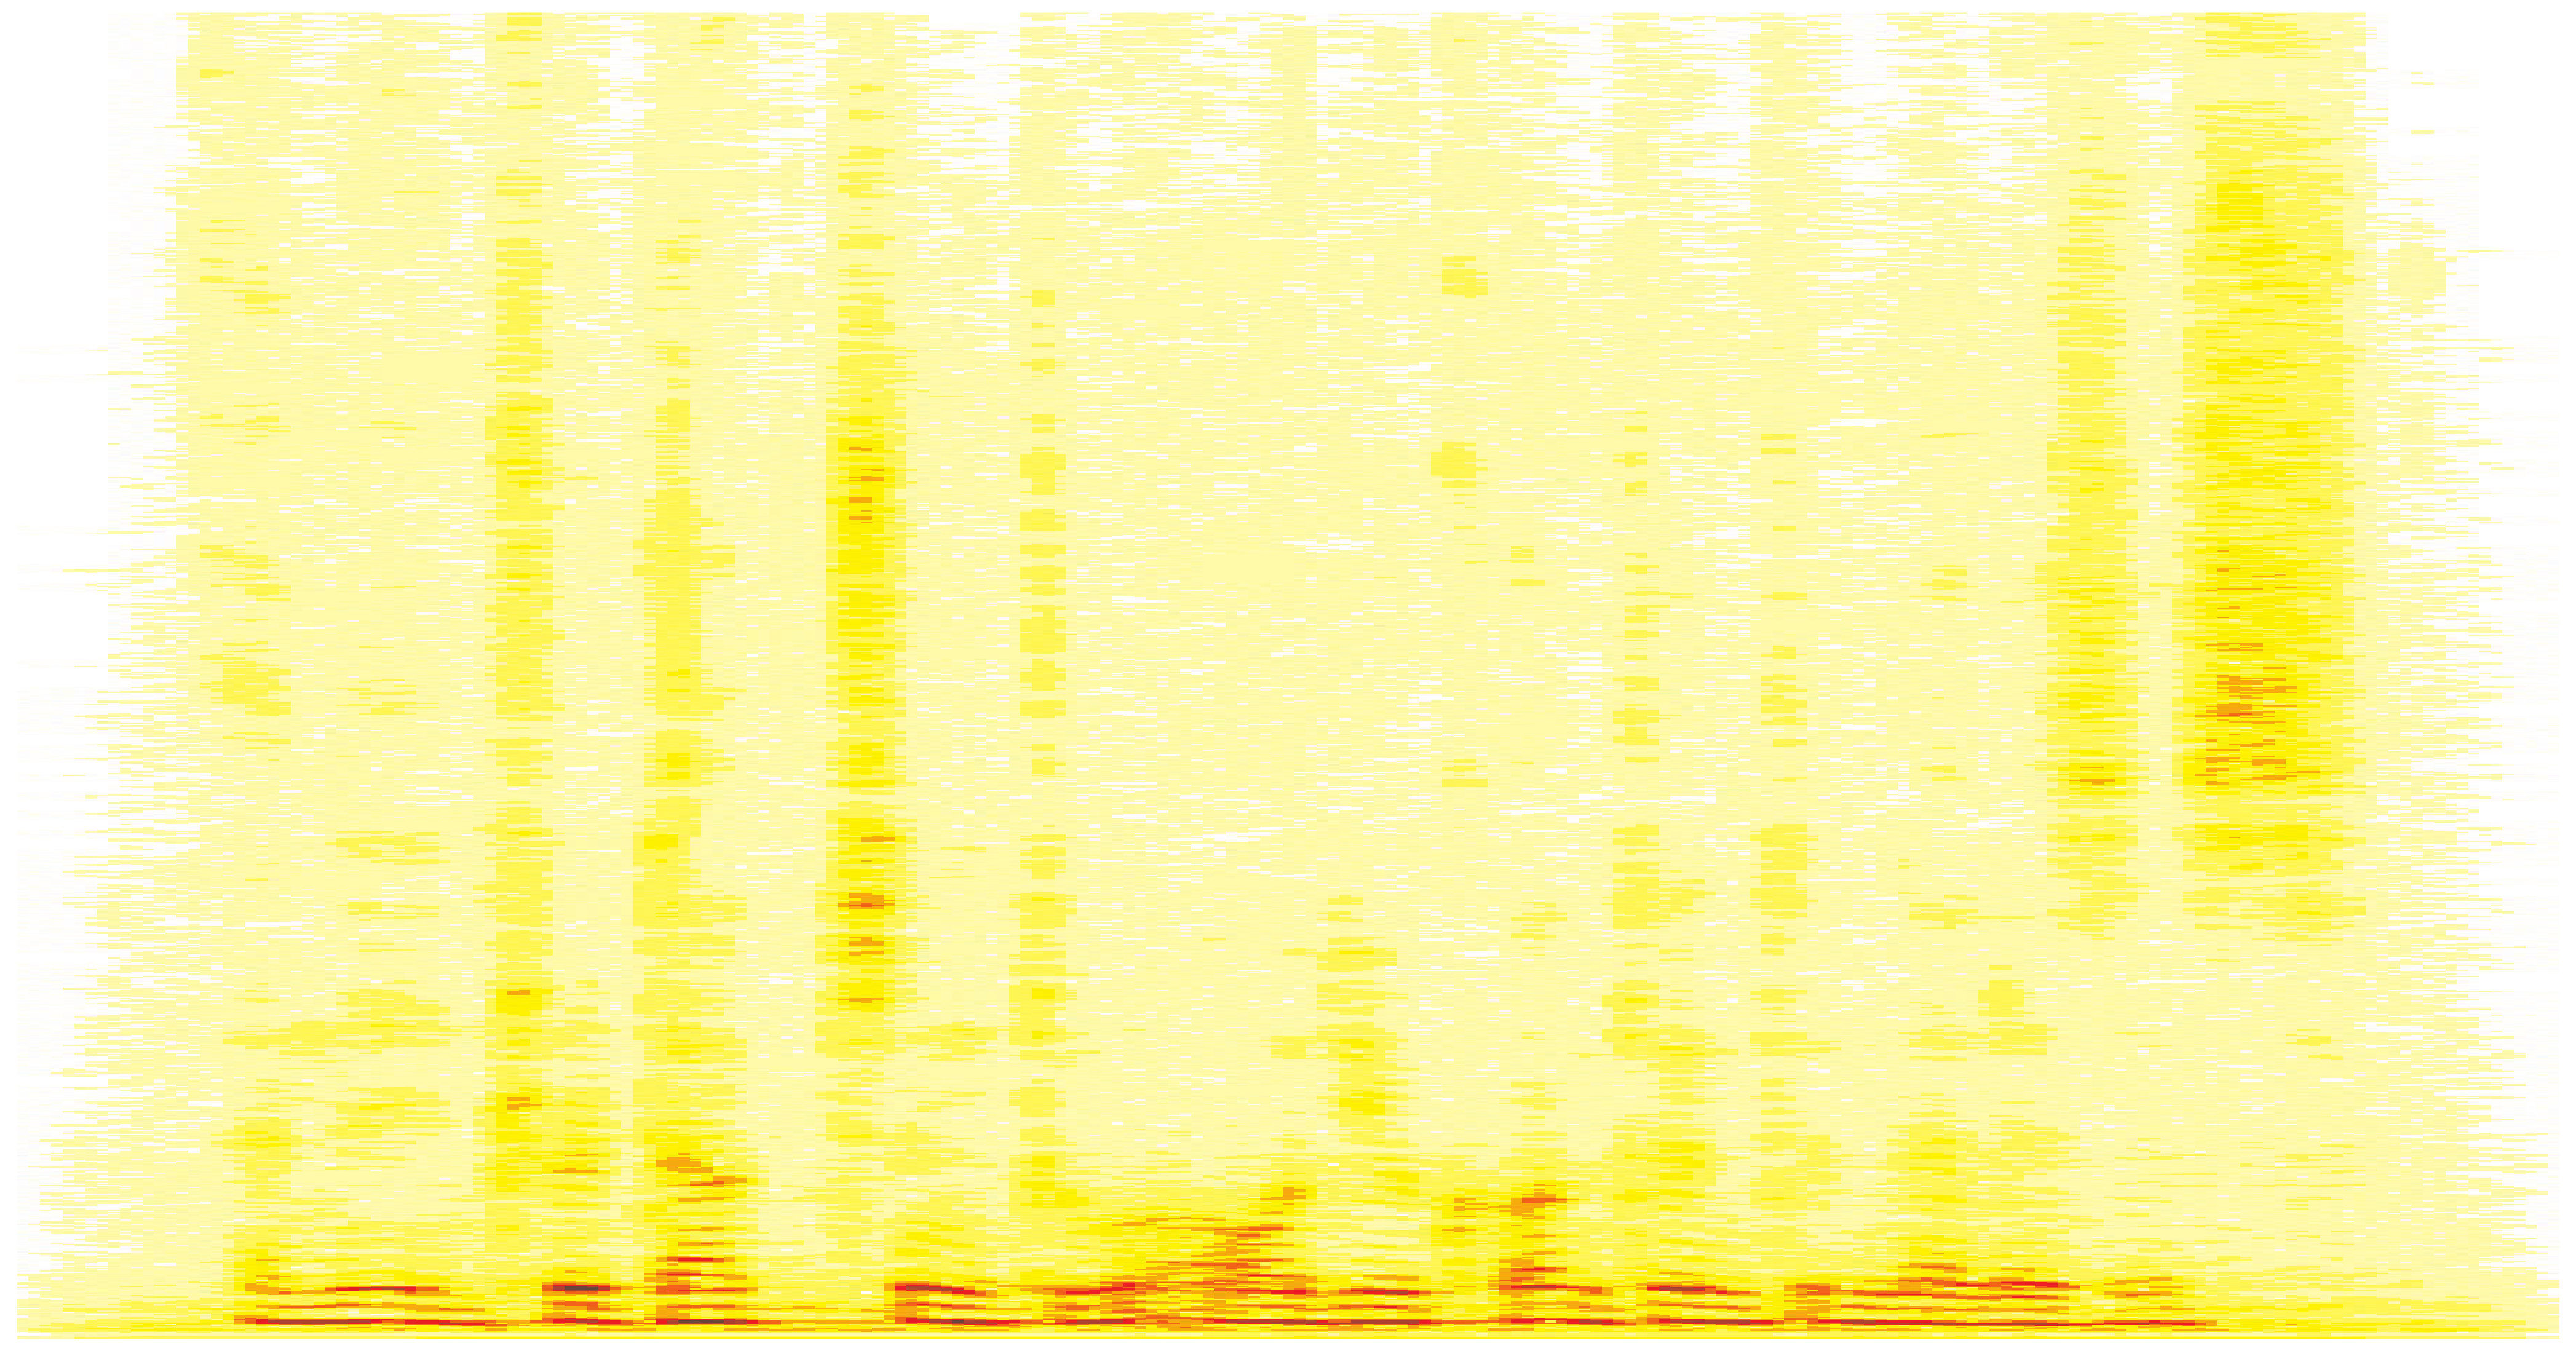
\includegraphics[width=\textwidth,height=3cm]{title}}

%%%%%%%%%%%%%%%%%%%%%%%%%%%%%%%%%%%%%%%%%%%%%%%%%%%%%%%%%%%%%%%%%%%%%%%%%%%%%%%%%%
%%%%%%%%%%%%%%%%%%%%%%%%%%%%%%%%%%%%%%%%%%%%%%%%%%%%%%%%%%%%%%%%%%%%%%%%%%%%%%%%%%
% colors
\definecolor{gtgold}{HTML}{96caff} %0e7eed {rgb}{0.88,0.66,1,0.06} [234, 170, 0]/256
\definecolor{darkgray}{rgb}{.1, .1, .25}
\definecolor{lightblue}{HTML}{0e7eed}
\definecolor{highlight}{rgb}{0, 0, 1} %_less!40

%%%%%%%%%%%%%%%%%%%%%%%%%%%%%%%%%%%%%%%%%%%%%%%%%%%%%%%%%%%%%%%%%%%%%%%%%%%%%%%%%%
%%%%%%%%%%%%%%%%%%%%%%%%%%%%%%%%%%%%%%%%%%%%%%%%%%%%%%%%%%%%%%%%%%%%%%%%%%%%%%%%%%
% relative paths
\graphicspath{{../ACA-Plots/graph/}}


%%%%%%%%%%%%%%%%%%%%%%%%%%%%%%%%%%%%%%%%%%%%%%%%%%%%%%%%%%%%%%%%%%%%%%%%%%%%%%%%%%
%%%%%%%%%%%%%%%%%%%%%%%%%%%%%%%%%%%%%%%%%%%%%%%%%%%%%%%%%%%%%%%%%%%%%%%%%%%%%%%%%%
% units
\setlength{\unitlength}{1mm}

%%%%%%%%%%%%%%%%%%%%%%%%%%%%%%%%%%%%%%%%%%%%%%%%%%%%%%%%%%%%%%%%%%%%%%%%%%%%%%%%%%
%%%%%%%%%%%%%%%%%%%%%%%%%%%%%%%%%%%%%%%%%%%%%%%%%%%%%%%%%%%%%%%%%%%%%%%%%%%%%%%%%%
% math
\DeclareMathOperator*{\argmax}{argmax}
\DeclareMathOperator*{\argmin}{argmin}
\DeclareMathOperator*{\atan}{atan}
\DeclareMathOperator*{\arcsinh}{arcsinh}
\DeclareMathOperator*{\sign}{sign}
\DeclareMathOperator*{\tcdf}{tcdf}
\DeclareMathOperator*{\si}{sinc}
\DeclareMathOperator*{\princarg}{princarg}
\DeclareMathOperator*{\arccosh}{arccosh}
\DeclareMathOperator*{\hwr}{HWR}
\DeclareMathOperator*{\flip}{flip}
\DeclareMathOperator*{\sinc}{sinc}
\DeclareMathOperator*{\floor}{floor}
\newcommand{\e}{{e}}
\newcommand{\jom}{\mathrm{j}\omega}
\newcommand{\jOm}{\mathrm{j}\Omega}
\newcommand   {\mat}[1]    		{\boldsymbol{\uppercase{#1}}}		%bold
\renewcommand {\vec}[1]    		{\boldsymbol{\lowercase{#1}}}		%bold

%%%%%%%%%%%%%%%%%%%%%%%%%%%%%%%%%%%%%%%%%%%%%%%%%%%%%%%%%%%%%%%%%%%%%%%%%%%%%%%%%%
%%%%%%%%%%%%%%%%%%%%%%%%%%%%%%%%%%%%%%%%%%%%%%%%%%%%%%%%%%%%%%%%%%%%%%%%%%%%%%%%%%
% media9
\newcommand{\includeaudio}[1]{
\href{run:audio/#1.mp3}{
\includegraphics[width=5mm, height=5mm]{graph/SpeakerIcon}}}

\newcommand{\includeanimation}[4]{{\begin{center}
                        \animategraphics[autoplay,loop,scale=.7]{#4}{animation/#1-}{#2}{#3}        
                        \end{center}
                        \addreference{matlab source: \href{https://github.com/alexanderlerch/ACA-Plots/blob/master/matlab/animate#1.m}{matlab/animate#1.m}}}
                        \inserticon{video}}
                        
%%%%%%%%%%%%%%%%%%%%%%%%%%%%%%%%%%%%%%%%%%%%%%%%%%%%%%%%%%%%%%%%%%%%%%%%%%%%%%%%%%
%%%%%%%%%%%%%%%%%%%%%%%%%%%%%%%%%%%%%%%%%%%%%%%%%%%%%%%%%%%%%%%%%%%%%%%%%%%%%%%%%%
% other commands
\newcommand{\question}[1]{%\vspace{-4mm}
                          \setbeamercovered{invisible}
                          \begin{columns}[T]
                            \column{.9\textwidth}
                                \textbf{#1}
                            \column{.1\textwidth}
                                \vspace{-8mm}
                                \begin{flushright}
                                     
\includegraphics[width=.9\columnwidth]{graph/question_mark}
                                \end{flushright}
                                \vspace{6mm}
                          \end{columns}\pause\vspace{-12mm}}

\newcommand{\toremember}[1]{
                        \inserticon{lightbulb}
                        }

\newcommand{\matlabexercise}[1]{%\vspace{-4mm}
                          \setbeamercovered{invisible}
                          \begin{columns}[T]
                            \column{.8\textwidth}
                                \textbf{matlab exercise}: #1
                            \column{.2\textwidth}
                                \begin{flushright}
                                     
\includegraphics[scale=.5]{graph/logo_matlab}
                                \end{flushright}
                                %\vspace{6mm}
                          \end{columns}}

\newcommand{\addreference}[1]{  
                  
                    \begin{textblock*}{\baselineskip }(.98\paperwidth,.5\textheight) %(1.15\textwidth,.4\textheight)
                         \begin{minipage}[b][.5\paperheight][b]{1cm}%
                            \vfill%
                             \rotatebox{90}{\tiny {#1}}
                        \end{minipage}
                   \end{textblock*}
                    }
                    
\newcommand{\figwithmatlab}[1]{
                    \begin{figure}
                        \centering
                        \includegraphics[scale=.7]{#1}
                        %\label{fig:#1}
                    \end{figure}
                    
                    \addreference{matlab source: \href{https://github.com/alexanderlerch/ACA-Plots/blob/main/matlab/plot#1.m}{plot#1.m}}}
\newcommand{\figwithref}[2]{
                    \begin{figure}
                        \centering
                        \includegraphics[scale=.7]{#1}
                        \label{fig:#1}
                    \end{figure}
                    
                    \addreference{#2}}  
                                    
\newcommand{\inserticon}[1]{
                    \begin{textblock*}{100mm}(14.5cm,7.5cm)
                        \includegraphics[height=.8cm,keepaspectratio]{graph/#1}
                    \end{textblock*}}            

%%%%%%%%%%%%%%%%%%%%%%%%%%%%%%%%%%%%%%%%%%%%%%%%%%%%%%%%%%%%%%%%%%%%%%%%%%%%%%%%%%
%%%%%%%%%%%%%%%%%%%%%%%%%%%%%%%%%%%%%%%%%%%%%%%%%%%%%%%%%%%%%%%%%%%%%%%%%%%%%%%%%%
% counters
\newcounter{i}
\newcounter{j}
\newcounter{iXOffset}
\newcounter{iYOffset}
\newcounter{iXBlockSize}
\newcounter{iYBlockSize}
\newcounter{iYBlockSizeDiv2}
\newcounter{iXBlockSizeDiv2}
\newcounter{iDistance}

\newcommand{\IEEELink}{https://ieeexplore.ieee.org/servlet/opac?bknumber=9965970}




\subtitle{module 7.3.3: fundamental frequency detection in monophonic signals}

%%%%%%%%%%%%%%%%%%%%%%%%%%%%%%%%%%%%%%%%%%%%%%%%%%%%%%%%%%%%%%%%%%%%%%%%%%%%
\begin{document}
    % generate title page
	{
\setbeamertemplate{headline}{} 
\setbeamertemplate{footline}{} 
\begin{frame}
    \titlepage
    %\vspace{-5mm}
\end{frame}
}
\addtocounter{framenumber}{-1}


    \section[overview]{lecture overview}
        \begin{frame}{introduction}{overview}
            \begin{block}{corresponding textbook section}
                    %\href{http://ieeexplore.ieee.org/xpl/articleDetails.jsp?arnumber=6331122}{Chapter 5~---~Tonal Analysis}: pp.~91--103
                    section~7.3.3
            \end{block}

            \begin{itemize}
                \item   \textbf{lecture content}
                    \begin{itemize}
                        \item   established approaches to monophonic pitch tracking in
                            \begin{itemize}
                                \item   time domain
                                \item   frequency domain
                            \end{itemize}
                    \end{itemize}
                \bigskip
                \item<2->   \textbf{learning objectives}
                    \begin{itemize}
                        \item   define the task of monophonic pitch tracking
                        \item   summarize the principles of time-domain $\hat{f}_0$-trackers and describe one approach in detail
                        \item   summarize the principles of frequency-domain $\hat{f}_0$-trackers and describe one approach in detail
                    \end{itemize}
            \end{itemize}
            \inserticon{directions}
        \end{frame}

    \section[intro]{introduction}

	\begin{frame}{fundamental frequency}{introduction}
        \begin{block}{\textbf{remember}}
            Fourier series: every (quasi-)periodic sound is a combination of sinusoidals with integer frequency ratios
        \end{block}
        \begin{eqnarray*}
            x(t) 	&\approx& x(t+\hat{T}_0)\nonumber\\
            x(t) &\approx& \sum\limits_{k=-\infty}^{\infty} a(k) \e^{\jom_0kt}\nonumber
        \end{eqnarray*}
        
		\begin{itemize}
			\item<2->[]	$\hat{f}_0$: musically, perceptually most ``relevant'' frequency
		\end{itemize}
        \only<2->{
        \begin{figure}[t]
            \centering
            
\includegraphics[scale=.7]{graph/pitch_harmonics}
        \end{figure}
        }
	\end{frame}
    
    \section[mono f0]{monophonic pitch tracking}
        \begin{frame}{pitch detection}{task definition}
            \begin{itemize}
                \item   detect the \textbf{fundamental frequency} $\hat{f}_0$
                \item   monophonic: only \textbf{one} fundamental frequency at a time
                \bigskip
                \item   related \textbf{subtasks}:
                    \begin{itemize}
                        \item   \textit{voice activity}: detect when there is no voice/no fundamental frequency
                        \item   \textit{note segmentation}
                            \begin{itemize}
                                \item   note start time and stop time
                                \item   average note frequency
                                \item   average note velocity
                                \item   vibrato detection
                            \end{itemize}
                        \item   frequency to \textit{pitch mapping}
                    \end{itemize}
            \end{itemize}
        \end{frame}

	\section[time domain]{time domain methods}
	\begin{frame}{monophonic fundamental frequency detection}{zero crossing rate}
        \vspace{-6mm}
        \begin{columns}
            \column{0.4\textwidth}
                \begin{itemize}
                    \item	\textbf{ZCR per block (bad)}
                        \begin{footnotesize}
                        \begin{equation*}
                            \hat{T}_0(n) = \frac{2\cdot \big(i_{\mathrm{e}}(n)-i_{\mathrm{s}}(n)\big)}{f_{\mathrm{S}}\cdot\sum\limits_{i=i_{\mathrm{s}}(n)}^{i_{\mathrm{e}}(n)}{\left|\sign \left[x(i)\right]-\sign \left[x(i-1)\right]\right|}} 
                        \end{equation*}
                        \end{footnotesize}
                    \item<2->	\textbf{average period length}
                        \begin{footnotesize}
                        \begin{equation*}
                            \hat{T}_0(n) = \frac{2}{\mathcal{Z}-1}\sum\limits_{j=0}^{\mathcal{Z}-2}{\Delta t_\mathrm{ZC}(j)}.
                        \end{equation*}
                        \end{footnotesize}
                    \item<3->	\textbf{variants}:
                        \begin{itemize}
                            \item	create distance histogram and choose maximum
                            \item	also use distances between local extrema
                        \end{itemize}
                \end{itemize}
            \column{.6\linewidth}
                \vspace{15mm}
                \figwithmatlab{F0Zcr}
        \end{columns}
	\end{frame}
	
	\begin{frame}{monophonic fundamental frequency detection}{auto correlation function}
		\vspace{-2mm}
        \only<1-2>{
        \begin{itemize}
            \item find \textbf{lag of ACF maximum}
                \begin{equation*}
                    r_{xx}(\eta,n) = \sum\limits_{i=i_{\mathrm{s}}(n)}^{i_{\mathrm{e}}(n)-\eta}{x(i)\cdot x(i+\eta)}
                \end{equation*}
                \begin{equation*}
                    \hat{T}_0(n) = \argmax\big(r_{xx}(\eta,n)\big)
                \end{equation*}
            \item<2->     \textbf{variants}:
                \begin{itemize}
                    \item<2>	center clipping
                            \begin{figure}
                                \centering
                                \begin{footnotesize}
	\begin{picture}(80,37)

	%%%%%%%%%%%%%%%%%%%%%%%%%%%
	% normal center clipping	
	\put(0, 21)
	{\vector(1,0){32}}
	\put(16, 5)
	{\vector(0,1){32}}
	
	\put(30, 23)
	{\text{{\shortstack[c]{$x$}}}}
	
	\put(8, 35)
	{\text{{\shortstack[c]{$\chi(x)$}}}}
	
	\put(2, 18)
	{\text{{\footnotesize{\shortstack[c]{$-c_\mathrm{L}$}}}}}
	
	\put(22, 18)
	{\text{{\footnotesize{\shortstack[c]{$+c_\mathrm{L}$}}}}}


	%%%%%%%%%%%%%%%%%%%%%%%%%%%
	% 3-level center clipping	
	\put(48, 21)
	{\vector(1,0){32}}
	\put(64, 5)
	{\vector(0,1){32}}

	\put(63.5, 13)
	{\line(1,0){1}}
	\put(63.5, 29)
	{\line(1,0){1}}
	
	\put(78, 23)
	{\text{{\shortstack[c]{$x$}}}}
	
	\put(56, 35)
	{\text{{\shortstack[c]{$\chi'(x)$}}}}
	
	\put(50, 18)
	{\text{{\footnotesize{\shortstack[c]{$-c_\mathrm{L}$}}}}}
	
	\put(70, 18)
	{\text{{\footnotesize{\shortstack[c]{$+c_\mathrm{L}$}}}}}
	
	\put(65, 13)
	{\text{{\footnotesize{\shortstack[c]{$-1$}}}}}
	
	\put(65, 29)
	{\text{{\footnotesize{\shortstack[c]{$+1$}}}}}
	
	
	% transfer functions

	\linethickness{0.5mm}	
	
	\put(8, 21)
	{\line(0,-1){8}}
	\put(24, 21)
	{\line(0,1){8}}
	\put(8, 13)
	{\line(-1,-1){8}}
	\put(24, 29)
	{\line(1,1){8}}
	\put(8, 21)
	{\line(1,0){16}}
	
	
	\put(56, 21)
	{\line(0,-1){8}}
	\put(72, 21)
	{\line(0,1){8}}
	\put(56, 13)
	{\line(-1,0){8}}
	\put(72, 29)
	{\line(1,0){8}}
	\put(56, 21)
	{\line(1,0){16}}

	\end{picture}
\end{footnotesize}

                                \label{fig:centerclipping}
                            \end{figure}
                   % \item<4->	pre-whitening: LP, spectral envelope estimation															
                \end{itemize}
        \end{itemize}
		}
        \only<3>{
            \figwithmatlab{F0Acf}
        }
            
	\end{frame}
	
	\begin{frame}{monophonic fundamental frequency detection}{average magnitude difference function}
        \only<1-2>{
        \begin{itemize}
            \item find \textbf{lag of AMDF minimum}
                \begin{equation*}
                    \mathrm{AMDF}_{xx}(\eta,n) = \frac{1}{i_{\mathrm{e}}(n)-i_{\mathrm{s}}(n)+1}\sum\limits_{i=i_{\mathrm{s}}(n)}^{i_{\mathrm{e}}(n)-\eta}{|x(i)- x(i+\eta)|} 
                \end{equation*}
            \item<2-> \textbf{variants}:
                \begin{itemize}
                    \item	AMDF-weighted ACF
                        \begin{equation*}
                            r_{xx}'(\eta,n) = \frac{r_{xx}(\eta,n)}{\mathrm{AMDF}_{xx}(\eta,n) + 1} 
                        \end{equation*}
                \end{itemize}
        \end{itemize}
        }
        \only<3>{
            \figwithmatlab{F0Amdf}
        }
	\end{frame}
	
    \section[frequency domain]{frequency domain methods}
	\begin{frame}{monophonic fundamental frequency detection}{harmonic product spectrum 1/2}
        \vspace{-13mm}
        \begin{columns}
            \column{0.4\textwidth}
                \vspace{4mm}
                \begin{equation*}\label{eq:hps}
                    X_{\mathrm{HPS}}(k,n) = \prod\limits_{j=1}^{\mathcal{O}}{|X(j\cdot k,n)|^2}
                \end{equation*}
                \begin{equation*}\label{eq:hps}
                    \hat{f}_0(n) = \argmax\big(X_{\mathrm{HPS}}(k,n)\big)
                \end{equation*}
                
                first published in the 1960s by Noll
            \column{0.6\textwidth}
                \figwithmatlab{F0HpsMethod}
		\end{columns}
        \vspace{-5mm}
        \phantom{\footfullcite{noll_pitch_1969}}
	\end{frame}
	
	\begin{frame}{monophonic fundamental frequency detection}{harmonic product spectrum 2/2}
		\figwithmatlab{F0Hps}
	\end{frame}
	
	\begin{frame}{monophonic fundamental frequency detection}{harmonic sum spectrum}
        \begin{itemize}
            \item   sum instead product sum
        \begin{equation*}\label{eq:hss}
            X_{\mathrm{HSS}}(k,n) = \sum\limits_{j=1}^{\mathcal{O}}{|X(j\cdot k,n)|^2} 
        \end{equation*}
        \bigskip

                \begin{itemize}
                    \item<1->   \textbf{advantage}
                        \begin{itemize}
                            \item   robust against missing harmonics
                        \end{itemize}
                    \item<1->   \textbf{disadvantage}
                        \begin{itemize}
                            \item   less pronounced peak
                        \end{itemize}
                \end{itemize}
        \end{itemize}
	\end{frame}
	
	\begin{frame}{monophonic fundamental frequency detection}{ACF of magnitude spectrum}
        \vspace{-3mm}
        \begin{columns}
        \column{.4\linewidth}
        \begin{footnotesize}
		\begin{equation*}
			r_{XX}(\eta,n) = \sum\limits_{k=-\mathcal{K}/2}^{\mathcal{K}/2-1}{|X(k,n)|\cdot |X(k+\eta,n)|}
		\end{equation*}
        \end{footnotesize}
		$\Rightarrow$ \textbf{detect maximum location}
        
        \column{.6\linewidth}
            \figwithmatlab{F0AcfOfFft}
        \end{columns}
	\end{frame}
	
	\begin{frame}{monophonic fundamental frequency detection}{cepstral pitch detection}
		\begin{enumerate}
			\item	compute cepstrum
			\item	detect periodicities
		\end{enumerate}
		\figwithmatlab{F0Cepstrum}
	\end{frame}
	
	\begin{frame}{monophonic fundamental frequency detection}{spectral maximum likelihood}
        \vspace{-2mm}
        \begin{itemize}
            \item   create \textbf{template matrix} with (smoothed) delta pulses for all possible frequencies
            
            \item<2->   compute the \textbf{cross correlation} ($lag=0$) between spectrum and all templates
            
            \item<3->   pick the result with the \textbf{highest correlation} $\Rightarrow$ frequency estimate % \footfullcite{cuadra_website}
        \end{itemize}
        \only<3->{
            \figwithmatlab{F0Template}%
        }
	\end{frame}
	
	\begin{frame}{monophonic fundamental frequency detection}{auditory-motivated pitch tracking 1/2}
		\begin{enumerate}
			\item	\textbf{filterbank} of band pass filters (e.g., mel scale)
			\item<2->	\textbf{HWR}
			\item<3->	\textbf{smoothing}
			\item<4->	within-band periodicity estimate (e.g. \textbf{ACF})
			\item<5->	\textbf{combination} of bands
		\end{enumerate}
	\end{frame}
	
	\begin{frame}{monophonic fundamental frequency detection}{auditory-motivated pitch tracking 2/2}
        \begin{columns}
        \column{.3\linewidth}
            \begin{enumerate}
                \item   filterbank output
                \bigskip
                \bigskip
                \bigskip
                \item   half wave rectification
                \bigskip
                \bigskip
                \bigskip
                \item   smoothed output
            \end{enumerate}
        \column{.7\linewidth}
            \vspace{-3mm}
            \figwithmatlab{F0Auditory}%
        \end{columns}
	\end{frame}
        
    \section{summary}
        \begin{frame}{summary}{lecture content}
            \begin{itemize}
                \item   \textbf{basic commonality}
                    \begin{itemize}
                        \item   all approaches look for \textbf{periodicity}
                            \begin{itemize}
                                \item   waveform similarity in time domain
                                \item   equidistant harmonics/peaks in freq domain
                            \end{itemize}
                    \end{itemize}
                \bigskip
                \item   \textbf{state-of-the-art}
                    \begin{itemize}
                        \item   despite the age of the presented methods, tweaked versions of the presented approaches are still often considered state-of-the-art
                        \item   combinations of different approaches can be robust
                    \end{itemize}
            \end{itemize}
            \inserticon{summary}
        \end{frame}
\end{document}
